\section{Модификация проекта «Изображение проекции полиэдра»}

\subsection*{Точная постановка задачи}
Назовём точку в пространстве «хорошей», если она находится на расстоянии строго меньше 1 от плоскости $\mathit x =2$ Модифицируйте эталонный проект таким образом, чтобы определялась и печаталась следующая характеристика полиэдра: сумма площадей проекций граней, центр и все вершины которых — «хорошие» точки.


\subsection*{Решение данной задачи}
Для выполнения поставленной задачи необходимо модифицировать код в файле $\texttt{common/polyedr.rb}$ 
Методы проверки центра грани, всех ее вершин и вычисление площади проекции грани выполняется в методе $\texttt{draw}$ класса $\texttt{Polyedr}$ в файле $\texttt{shadow/polyedr.rb}$:


\begin{small}
\begin{verbatim}
class Polyedr 
  attr_reader :edges, :facets, :total_area
  def initialize(file)
    @total_area = 0.0
    ...
    nf.times do
      ...
     @total_area += facet.area if facet.all_good?() 
      end
    puts "Нужная сумма: #{@total_area}"
    end
  end
end
\end{verbatim}
\end{small}

 \subsection*{Модификация кода}

В файле $\texttt{common/polyedr.rb}$ добавим метод $\texttt{is\_good?}$, который позволит проверять точку на расстояние от плоскости $\mathit x=2$. Расстояние от точки $\mathit{M(M_{x},~M_{y},~M_{z})}$ для плоскости, заданной уравнением $\mathit{Ax+By+Cz+D=0},$ от точки вычисляется по формуле: 
$$ \mathit{d=\frac{|AM_{x}+BM_{y}+CM_{z}+D|}{\sqrt{A^2+B^2+C^2}}}.$$
Так как в условии задачи плоскость задана уравнением $\mathit x=2$, то уравнение принимает вид
$$ \mathit{d=\frac{|M_{x}+0+0-2|}{\sqrt{1+0+0}}=|M_{x}-2|}.$$
Если расстояние больше, либо равно единице, то метод вернет $\texttt{false}$, иначе, метод вернет $\texttt{true}$ :
\begin{small}
\begin{verbatim}
class R3 
  ...
  def is_good?()
    (x - 2).abs < 1
  end
end
\end{verbatim}
\end{small}

Затем добавим методы в класс $\texttt{Facet}$. Метод $\texttt{all\_good?}$ возвращает $\texttt{true}$, когда все вершины грани и ее центр ~--- хорошие точки, и $\texttt{false}$, когда не все. Координаты центра грани находятся с помощью метода $\texttt{center}$, который используется в файле $\texttt{shadow/polyedr.rb}$ эталонного проекта.
\begin{small}
\begin{verbatim}
class Facet 
  ...
  def all_good?()
    @vertexes.all?{|i| i.is_good?()} and center.is_good?()
  end
  ...
end
\end{verbatim}
\end{small}

Далее напишем вспомогательный метод $\texttt{triangle\_area(a, b, c)}$, который считает площадь треугольника, заданного вершинами $\texttt{a, b}$ и $\texttt{c}$. В данном методе используется формула вычисления площади треугольника по вершинам при помощи определителя матрицы:

$$ \mathit S = \frac{1}{2}\begin{vmatrix}
a_{x}-c_{x} & a_{y}-c_{y} \\ 
b_{x} - c_{x} & b_{y} - c_{y}
\end{vmatrix} .$$

\begin{small}
\begin{verbatim}
class Facet
  ...
  def triangle_area(a, b, c)
    0.5*((a.x-c.x)*(b.y-c.y)-(a.y-c.y)*(b.x-c.x)).abs
  end
end
\end{verbatim}
\end{small}

Затем реализуем метод $\texttt{area}$, который будет основным для подсчета площади проекции грани. Данный метод будет базироваться на вспомогательном методе $\texttt{triangle\_area(a, b, c)}$, где в качестве агрумента $\texttt{с}$ будет передаваться центр грани. Циклом пройдем по всем вершинам и просуммируем площади всех треугольников, из которых состоит грань, тем самым получим площадь проекции грани.

\begin{small}
\begin{verbatim}
class Facet
  ...
  def area
    area = 0.0; c = center
    (-1...@vertexes.size - 1).each do |i|
      area += triangle_area(@vertexes[i], @vertexes[i + 1], c)
    end
    area
  end
  ...
end
\end{verbatim}
\end{small}

На этом решение поставленной завершено. Пример работы программы 
с модифицированным файлом $\texttt{test3.geom}$ можно увидеть на рис.2 и его содержание представленно ниже.
\begin{figure}[ht!]
\begin{center}
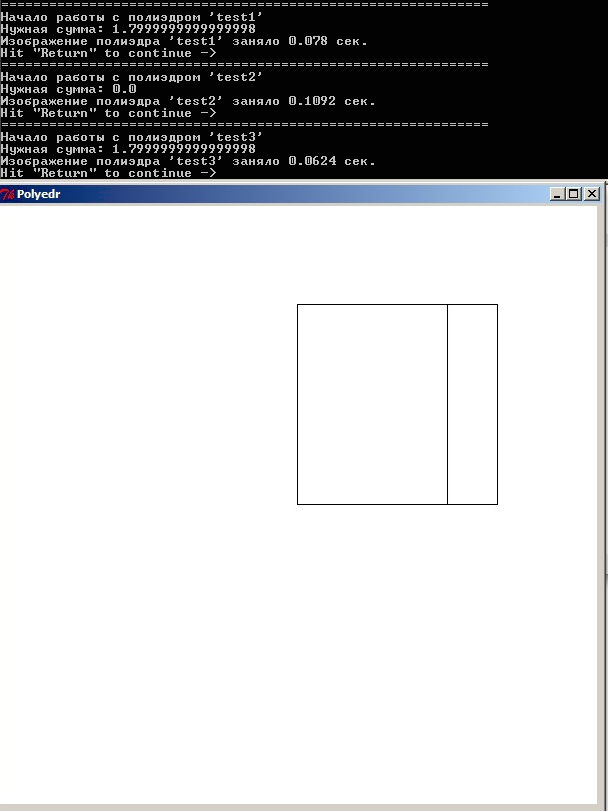
\includegraphics[width=0.8\hsize]{images/shadow}
\end{center}
\caption{Работа программы «Изображение проекции полиэдра»}
\end{figure}
\newpage\begin{small}
\begin{verbatim}
1	0	0	0
10 3 12
2.0 0 0
2.0 2 0
1.5 0 2
1.5 2 2
1.1 0 0
1.1 2 0
0 0 0
0 2 0
1.5 0 2
1.5 2 2
4 1 2 4 3
4 5 6 4 3
4 7 8 4 3

\end{verbatim}
\end{small}



